\section{Personagens}

\subsection{Introdução}
O jogo apresentará duas classes de dificuldades ao personagem principal 
(ou jogador): de percurso e de inimigos. As dificuldades de percurso serão 
aquelas apresentadas pelo ambiente e que exigirá a habilidade de locomoção 
do personagem, tal como salto ou desvio de obstáculos. As dificuldades 
de inimigos serão aquelas que exigirão a habilidade de ataque e defesa 
do personagem quando em confronto com um inimigo.

Nas seções a seguir são apresentadas as formas de controle dos estados 
do personagem principal, os inimigos e suas respectivas características 
e, por fim, o cenário e seus desafios.

\subsection{Estados do Personagem Principal}
Na primeira fase do jogo, haverá duas barras para que o jogador possa 
controlar os estados do per-sonagem principal, ou seja, a condição física 
dele: a barra de vida e a barra de energia.
 
\subsubsection{Barra de Vida}
A barra de vida exibe o nível de vitalidade do personagem principal. 
A Figura 1 apresenta um esboço desta barra, que começa completa, com
100 pontos percentuais. São dois os fatores que influenciarão no 
decaimento do nível: ataques sofridos e barra de energia vazia. Os ataques 
sofridos condizem com os ata-ques dos animais que o personagem encontrará
nos cenários da primeira fase. O valor que será decremen-tado da barra de 
vida dependerá da força de ataque do animal em específico. Sobre a barra de 
energia vazia e a forma de recuperação da força vital do personagem, estas
são tratadas na subseção a seguir.

\begin{figure}[!ht]
 \centering
 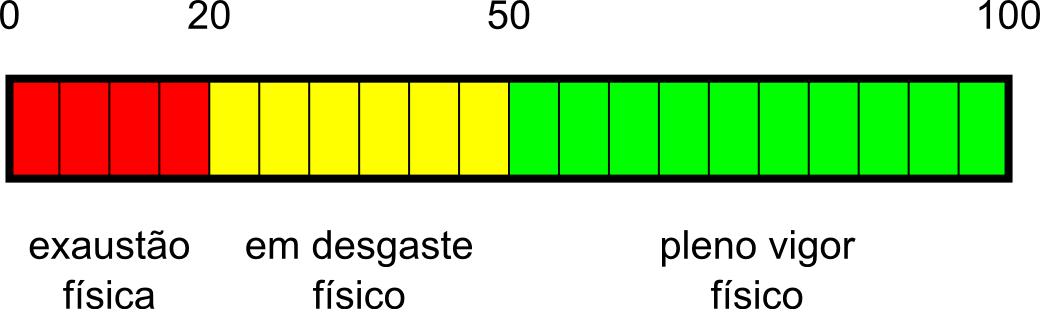
\includegraphics[scale=3]{BarraDeEnergia.png}
 \caption{Esboço das barras de vida (acima) e energia (abaixo).}
 \label{img:energia}
\end{figure}

\subsubsection{Barra de Energia}
A barra de energia exibe o nível de resistência física do personagem principal, 
ou seja, a capacidade dele para desenvolver um esforço físico. A Figura 1 apresenta 
um esboço desta barra, que inicia cheia. No intervalo de 50 a 100, destacado em 
verde, o personagem estará em pleno vigor físico. Ele conseguirá correr e pular 
alto ou longas distâncias. No intervalo de 20 a 50, destacado em amarelo, o 
personagem começará a sofrer um desgaste físico. Ele passará a correr cada vez 
mais lento e a saltar alturas e distâncias cada vez menores até chegar à exaustão 
física – a função para controle da capacidade de esforço físico do persona-gem é 
apresentada no Gráfico 1. No intervalo de 0 a 20, o personagem já não conseguirá 
mais correr e nem pular, apenas andar.

\begin{figure}[!ht]
 \centering
 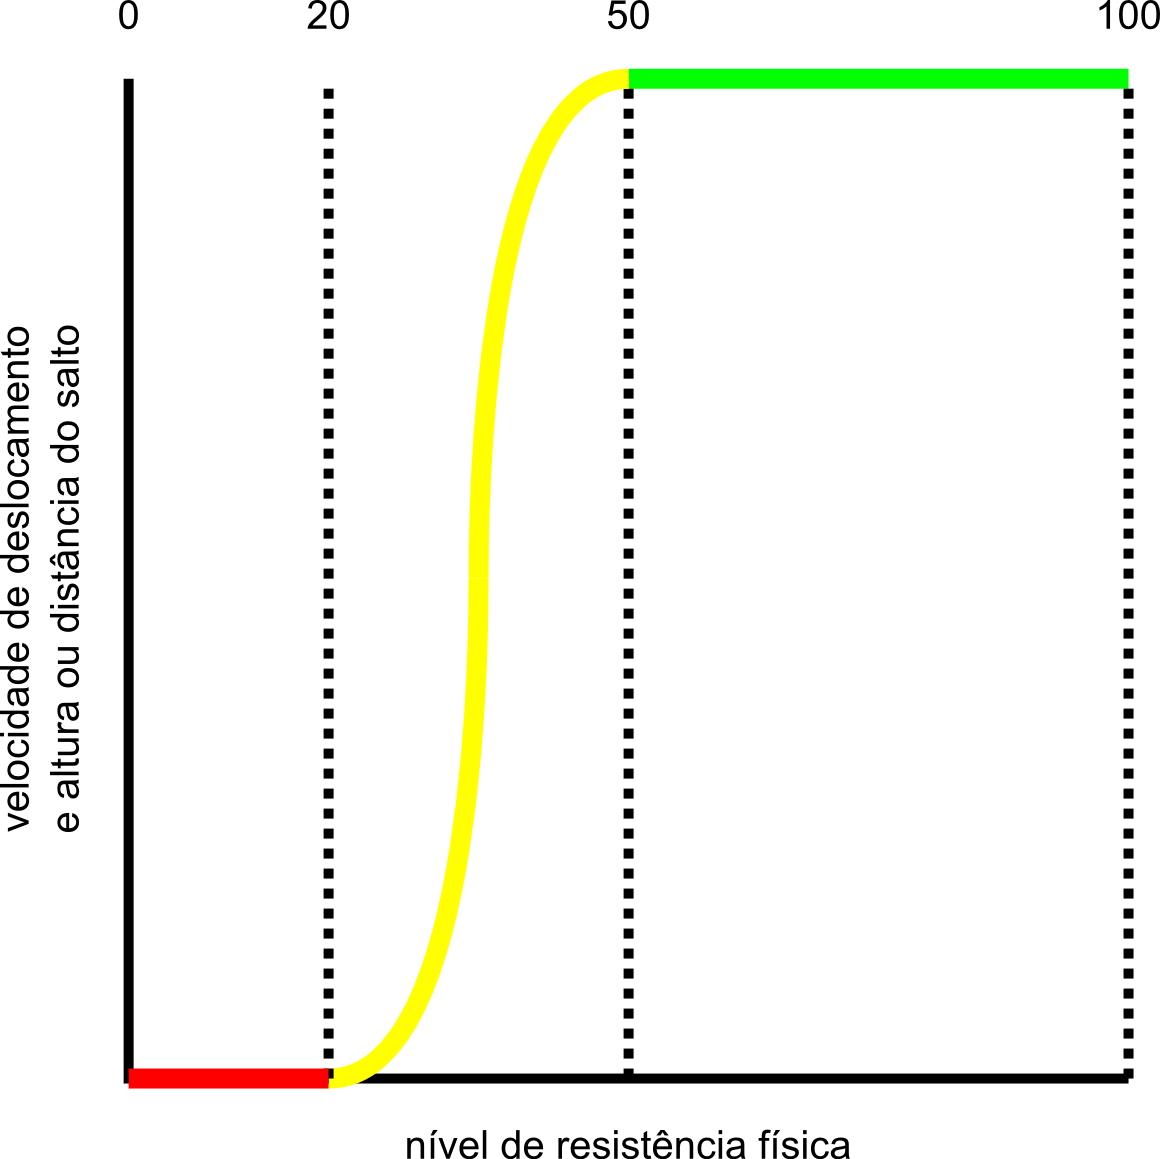
\includegraphics[scale=2.5]{VelocidadeDeDeslocamentoEPulo.png}
 \caption{Relação entre a capacidade de esforço físico e a energia do personagem.}
 \label{img:velocidade}
\end{figure}

Os fatores que influenciarão no decaimento do nível de resistência física 
do personagem são: deslocamento, pulo e golpe. No deslocamento, o nível de 
energia deverá reduzir linearmente em função da distância percorrida pelo 
personagem. A cada pulo ou golpe realizado pelo personagem será decrementado 
ao nível de energia 1 e 1/2 ponto percentual, respectivamente. Se a barra de 
energia estiver vazia, estes fatores deverão interferir, na mesma proporção, 
no nível de vitalidade do personagem. Para elevar ambos os níveis de 
resistência física e de vitalidade, o personagem deverá matar e, em 
seguida, se alimentar dos animais que ele encontrará pelo caminho. Cada 
animal tem o seu valor energético específico.

\subsection{Personagens e Inimigos}
Na primeira fase, os inimigos do personagem principal serão os animais da floresta. 
Haverá cinco espécies de animais: cobra, urso, abelha, jacaré e tigre. Cada espécie 
terá suas características específicas. Estas são apresentadas na Tabela 1, em que K 
é um valor constante e p.p. é a abreviação de pontos percentuais.

\begin{figure}[!ht]
 \centering
 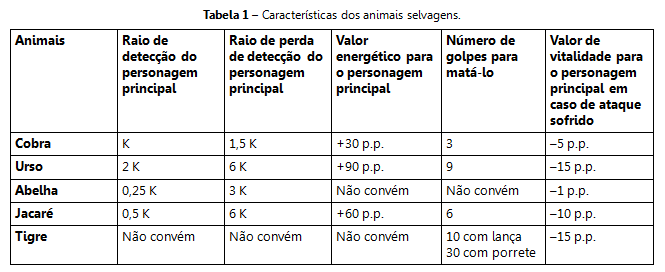
\includegraphics[scale=1]{tabela.png}
 \caption{}
 \label{img:tabela}
\end{figure}
